\chapter{Training}

	\section{Training Set}

	\section {Preprocessing and Data Augmentation}




		\subsection{Normalization}
Research \cite{lecun_norm} has shown that neural networks perform consistently better when the input data is normalized, that is, when the data is has zero mean and unit variance. This is achieved by performing almost the same thing that happens in the Batch Normalization layer, only that no additional transformation is applied.

		\subsection{Cropping and Rotation}
One problem with training deep Neural Networks is the immense amount of data required. Common image datasets such as MNIST\footnote{\url{http://yann.lecun.com/exdb/mnist/}}, CIFAR-10/100\footnote{\url{https://www.cs.toronto.edu/~kriz/cifar.html}} and LSVRC-2010 (ImageNet)\cite{ILSVRC} contain 10,000 to 1.3 million images. Such numbers are absolutely out of reach for most biomedical applications as the data required is highly specialized. Creating the labelled data for this thesis took 30 - 45 minutes per image, making it infeasible to manually create a large training set.

To nonetheless train a network to segment such images, \textit{data augmentation} can be used to artificially increase the number of samples. An easy way to multiply the number of samples eightfold is to flip all images only vertically, followed by rotations of both the original images and their flipped counterparts by $90^{\circ}$, $180^{\circ}$ and $270^{\circ}$, as this yields all possible combinations that are possible by flipping and rotating in $90^{\circ}$ steps.

		\subsection{Elastic Deformation}
Another data augmentation technique is \textit{Elastic deformation} \cite{elastic}, which calculates a new image from an existing one by sampling random new positions for each pixel in the original image uniformly and multiplies them with a force parameter $\alpha$. Afterwards, the new coordinates are additionally smoothed by a Gaussian filter with standard deviation $\sigma$. The resulting image is a slightly distorted image, and if $\alpha$ and $\sigma$ are chosen appropriately, the resulting images are plausible enough to count as ``new'' samples to train on (see figure \ref{fig:elastic}). For the work in thesis, the variables were set to $\alpha = 200$ and $\sigma = 10$.


\begin {figure}[!ht]
	\begin{center}
		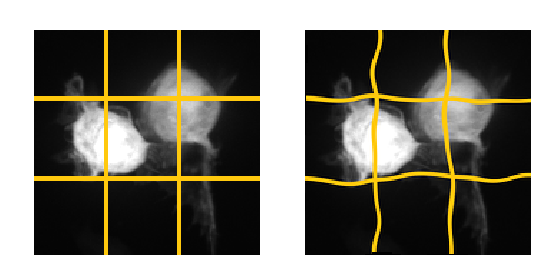
\includegraphics[scale=0.80]{img/fig_elastic.png}
	\end{center}
	\caption[]{\textbf{Left:} Input image with superimposed grid. \textbf{Right:} Elastic deformation with $\alpha = 100$ and $\sigma = 10$.}
	\label{fig:elastic}
\end {figure}

	\section {Training Algorithms and Parameters}
	\textbf{TODO:} put ReLU, leaky ReLU, parametric ReLU and ELU here!\\ Include XAVIER init.. is Xavier ok with ReLU? "He et al. 2015", https://www.youtube.com/watch?v=gYpoJMlgyXA
	
	\section{Non-convex Functions and Momentum}

	\section {Pseudo-Labelling}

		\subsubsection {The Cluster Assumption}

	\section {Validation}
		
		\subsection{Early Stopping}